\documentclass{article}

%使用ctex宏包支持中文
\usepackage{ctex}

%插入图片需要使用的包
\usepackage{graphicx}

%设置图片保存的路经
\graphicspath{{images/}}

%保证插入的图片严格放在指定位置
\usepackage{float}

%设置页边距
\usepackage{geometry}
\geometry{a4paper , scale = 0.85}

%设置页眉页脚
\usepackage{fancyhdr}
\pagestyle{fancy}
\lhead{2018年}
\chead{图像复原实验报告}
\rhead{2015011006 王道烩}
\lfoot{}
\cfoot{\thepage}
\rfoot{}


\begin{document}
	%制作标题页
	\begin{center}
		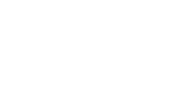
\includegraphics[height = 8cm]{blank.png}
		
		{\heiti \zihao{-0} 图像复原报告}
		
		\vspace{10cm}
		
		{\kaishu \zihao{2}  姓名:王道烩 \\ 班级: 无52 \\ 学号:2015011006\\}
	\end{center}
	
	\newpage
	\section{实验目的}
		\begin{enumerate}
			\item 了解常见的图像退化形式。
			\item 了解常见的图像复原方法。
			\item 掌握正弦噪声干扰和运动模糊图像的复原方法。
		\end{enumerate}
	\section{实验环境}
		\begin{enumerate}
			\item 操作系统:ubuntu16.04 LTS
			\item 编程语言:Python 3.5
			\item 工具包:numpy、opencv 3.2.1
		\end{enumerate}
	\section{有正弦干扰的图像}
		\subsection{数学原理}
			由老师上课讲的二维正弦干扰模式为:
			$$n( x , y) = Asin(u_0x+v_0y)$$
			其傅丽叶变换为:
			$$ N(u , v ) = \frac{-jA}{2}[\delta(u-\frac{u_0}{2\pi} , v - \frac{v_0}{2\pi}) - \delta(u + \frac{u_0}{2\pi} , v + \frac{v_0}{2\pi})]$$
			上式表明其频谱在$(\frac{u_0}{2\pi} , \frac{v_0}{2\pi})$和$(-\frac{u_0}{2\pi} , -\frac{v_0}{2\pi})$处出现脉冲。在显示时会出现两个亮点。因此解决方案就是在这两个脉冲处设置一个mask,将这两个亮点去除。
		\subsection{实验结果}
			在原图的频谱中将滤波器画上如下图 \ref{滤波器范围} 所示:
			\begin{figure}[H]
				\centering
				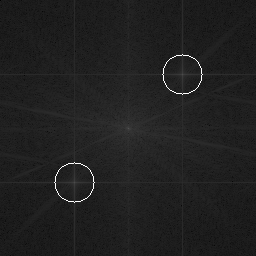
\includegraphics[scale = 0.7]{fft_masked.png} \label{滤波器范围}
				\caption{滤波器大致范围}
			\end{figure}
			
			经过滤波器作用之后的频谱如下所示
			\begin{figure}[H]
				\centering
				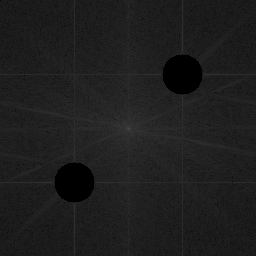
\includegraphics[scale = 0.7]{fft_newimg.png} 
				\caption{输出图片频谱}
			\end{figure}
			
			最终的复原图像如下:
			\begin{figure}[H]
				\centering
				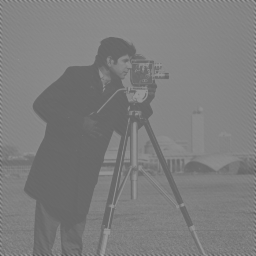
\includegraphics[scale = 0.7]{new.png} 
				\caption{修复后的图片}
			\end{figure}
			
			当增大滤波器半经时,可以看到振铃效应,如下图:
			\begin{figure}[H]
				\centering
				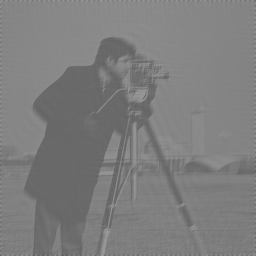
\includegraphics[scale = 0.7]{振铃.png} 
				\caption{振铃现象}
			\end{figure}
		
	\section{运动模糊无噪声的图像}
		%\subsection{数学原理}
		\subsection{逆滤波}
			考虑噪声时,有
			$$ G(u,v) = H(u,v) F(u,v) +N(u,v)$$	
			
			所以有:
			$$ \hat{F}(u ,v) = F(u ,v) + \frac{N(u ,v)}{H(u ,v)}$$	
			
			但是实际上如果$H(u,v)$很小或者为0时,则导致复原结果不稳定。且如果$\frac{N(u ,v)}{F(u,v)}$值过大,会掩盖真实信息。所以实际中采取的方法是:
			\begin{equation}
			M(u , v) = \left\{
				\begin{array}{lr}
					\frac{1}{H(u ,v)} & u^2 + v^2 \le \omega_0 \\
					1 & u^2+v^2 > \omega_0
				\end{array}
				\right.
			\end{equation}

		在运动模糊这一部分由课堂上老师讲的原理有:
		$$H(u ,v) = \int_{0}^{T}{e^{-j2\pi[ux_0(t) + vy_0(t)]}}dt = \frac{T}{\pi(uc+vb)}sin[\pi(uc+vb)]e^{-i\pi(uc+vb)}$$
		
		所以直接作用到图片上即可。但是本人在实验中发现了一些问题:
		首先由于模糊实在原图的频谱上叠加一个正弦波,所以会存在非常多的零点。原始图像的频谱如下图所示:
		
		\begin{figure}[H]
			\centering
			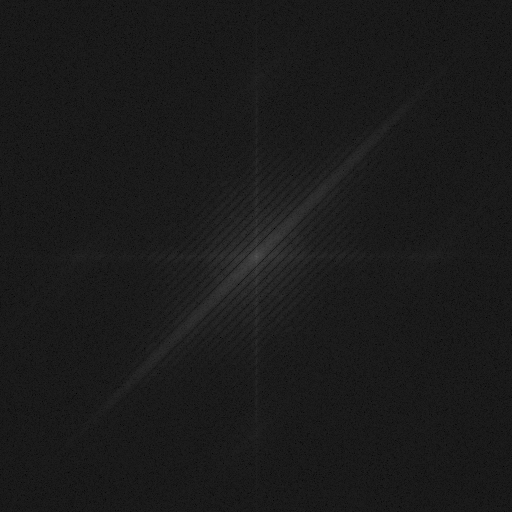
\includegraphics[scale = 0.5]{original_fft.png}
			\caption{原始图像频谱}
		\end{figure}
		
		如果直接用H去除的话,会在零点处出现非常大的值,直接使用H除得到的频谱如下:
		
		\begin{figure}[H]
			\centering
			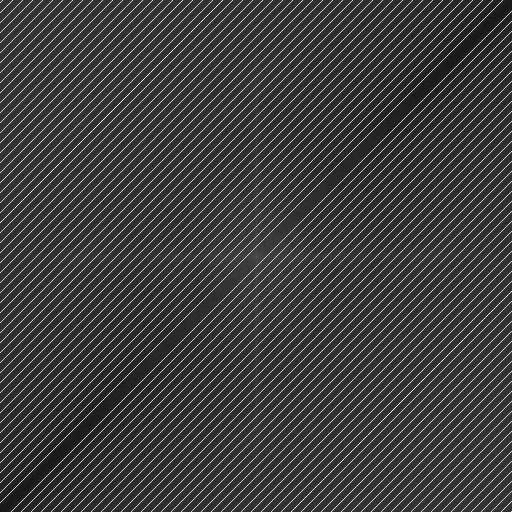
\includegraphics[scale = 0.5]{no_process.png}
			\caption{直接除以H得到的频谱}
		\end{figure}
		
		对于这样的问题,本人通过观察发现这些非常大的值只会发生在特定的点上。所以本人的解决方法是遍历整个频谱,如果这个位置上的值比中心点的值大非常多的话,就可以判断这个点为坏点。然后用这个点的周围的四个点平均值替换这个点的值。通过这样的处理得到的频谱如下:
		
		\begin{figure}[H]
			\centering
			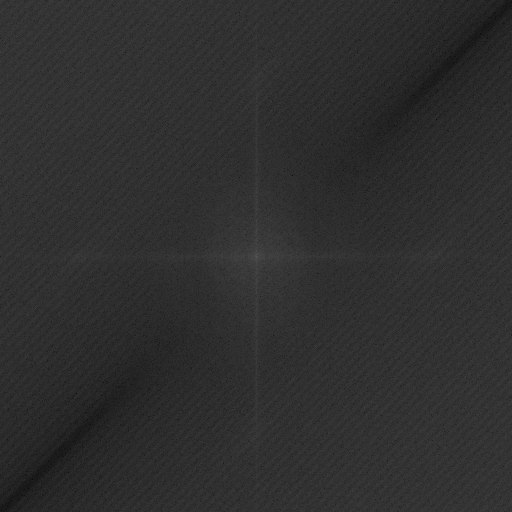
\includegraphics[scale = 0.5]{process.png}
			\caption{处理后的频谱}
		\end{figure}
		
		可以观察到这样得到的频谱得到了非常大的改善。所以最终的复原图像如下所示:
		
		\begin{figure}[H]
			\centering
			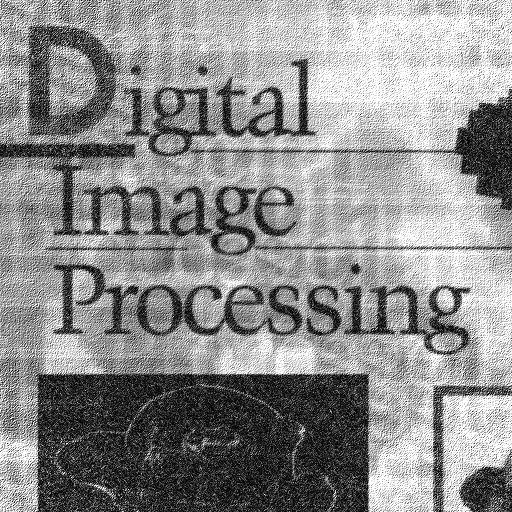
\includegraphics[scale = 0.5]{result1.png}
			\caption{逆滤波复原最终结果}
		\end{figure}
		
		可以看到基本恢复了原始图像,但是存在着一些颗粒噪声。
	
		\subsection{维纳滤波}
		由老师上课推倒的结果有:
		$$\hat{F}(u,v) = [\frac{1}{H(u ,v)}\frac{|H(u,v)|^2}{|H(u,v)|^2+s[\frac{S_n(u,v)}{S_f(u ,v)}]}]G(u ,v)$$
		
		但是实际上$S_n(u , v)$ 和 $S_f(u ,v)$很少是已知的,因此上式常用下式近似:
		$$ \hat{F}(u ,v) = [\frac{1}{H(u ,v)}   \frac{|H(u ,v)|^2}{|H(u,v)|^2 + K}]G(u ,v)$$
		
		K为噪声和信号的功率密度比。
		
		本人从直观上理解,如果$H(u ,v)$的值比较小的时候,那么多出来的那一向也会比较小,这样就可以减轻零点带来的效应。当$H(u,v)$比较大的时候,多出来的那一向几乎为1,没有什么影响。
		最终实验得到的结果如下:
		
		\begin{figure}[H]
			\centering
			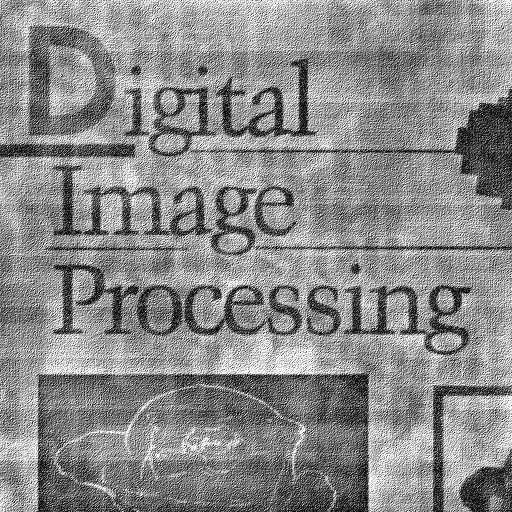
\includegraphics[scale = 0.5]{result2.png}
			\caption{维纳滤波最终结果}
		\end{figure}
	\section{运动模糊有噪声的图像}
	
	这一部分本人经过多次尝试,均不能取得比较好的复原结果。下面就原因进行简要分析:
	
	首先我将原图的频谱画出如下图所示:
	\begin{figure}[H]
		\centering
		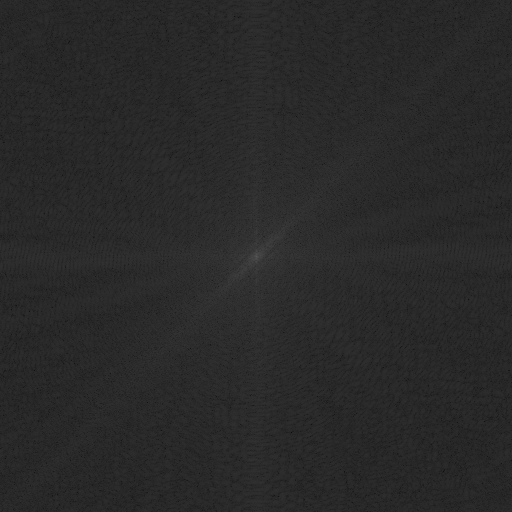
\includegraphics[scale = 0.5]{noise_fft.png}
		\caption{噪声存在的图像频谱}
	\end{figure}
	
	通过观察能够看出,这张图片的频谱和无噪声的那张图片最大的区别就是没有明显的被Sa函数叠加的样子。这样就使后面使用直接逆滤波进行处理有些问题。对图像进行逆滤波处理得到的频谱如下所示:
	\begin{figure}[H]
		\centering
		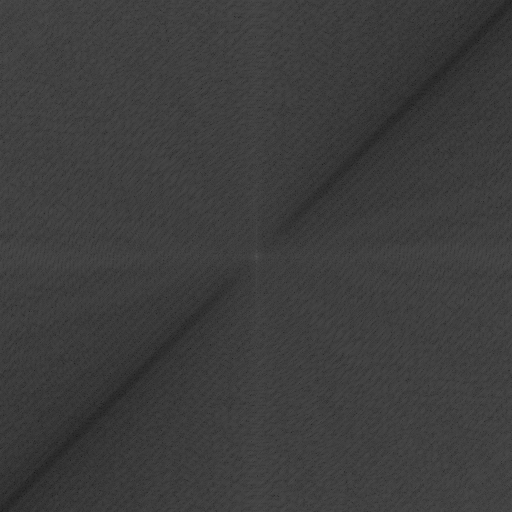
\includegraphics[scale = 0.5]{noise_processed.png}
		\caption{噪声图像处理过后的频谱}
	\end{figure}
	
	最终输出的图片如下所示:
	\begin{figure}[H]
		\centering
		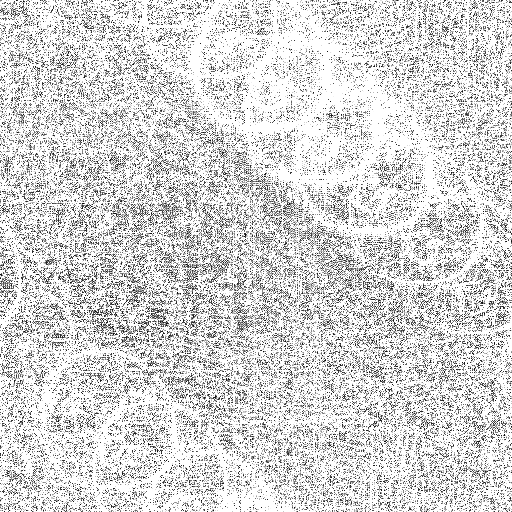
\includegraphics[scale = 0.5]{noise_result1.png}
		\caption{噪声图像逆滤波结果}
	\end{figure}
	
	同样,本人使用维纳滤波器并不断尝试各种K值,但是最终结果都不理想。最终结果如下:
	\begin{figure}[H]
		\centering
		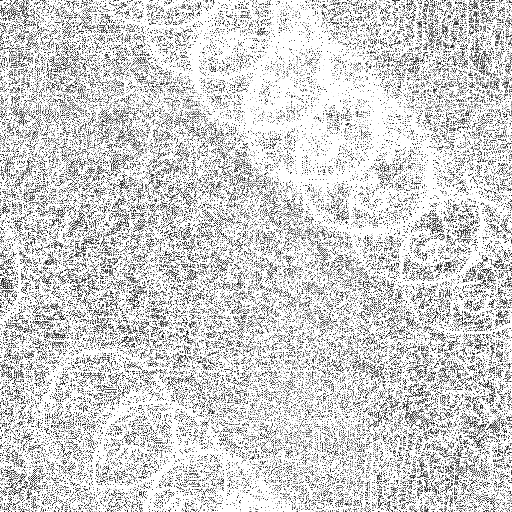
\includegraphics[scale = 0.5]{noise_result2.png}
		\caption{噪声图像维纳滤波结果}
	\end{figure}
	\section{总结}
	通过本次实验,对图像复原所使用的逆滤波以及维纳滤波原理有了更加深刻的理解。同时掌握了运动模糊图像复原的方法。
	
	但是同样存在这非常大的改进的地方。当运动图像存在这噪声干扰的时候,如果对于噪声的信息没有任何先验知识的话,那么最后恢复出来的图像效果会非常差。本人通过观察噪声污染后的图片的频谱,发现噪声非常厉害,完全将原始运动的痕迹给摸去。而且还在图片上面画一个笑脸。。这同时也体现了图像复原对于先验只是是非常依赖的。
	
	谢谢助教、老师在这一学期的细心指导,让我学到非常多的东西。希望助教、老师身体健康,工作顺利!!!
\end{document}



